\documentclass[bachelor, och, labwork]{shiza}

\usepackage{subfigure}
\usepackage{tikz,pgfplots}
\pgfplotsset{compat=1.5}
\usepackage{float}

\usepackage{titlesec}
\setcounter{secnumdepth}{4}
\titleformat{\paragraph}
{\normalfont\normalsize}{\theparagraph}{1em}{}
\titlespacing*{\paragraph}
{35.5pt}{3.25ex plus 1ex minus .2ex}{1.5ex plus .2ex}

\titleformat{\paragraph}[block]
{\hspace{1.25cm}\normalfont}
{\theparagraph}{1ex}{}
\titlespacing{\paragraph}
{0cm}{2ex plus 1ex minus .2ex}{.4ex plus.2ex}

% --------------------------------------------------------------------------%


\usepackage[T2A]{fontenc}
\usepackage[utf8]{inputenc}
\usepackage{graphicx}
\graphicspath{ {./images/} }
\usepackage{tempora}

\usepackage[sort,compress]{cite}
\usepackage{amsmath}
\usepackage{amssymb}
\usepackage{amsthm}
\usepackage{fancyvrb}
\usepackage{listings}
\usepackage{listingsutf8}
\usepackage{longtable}
\usepackage{array}
\usepackage[english,russian]{babel}

\usepackage[colorlinks=true]{hyperref}
\usepackage{url}

\usepackage{underscore}
\usepackage{setspace}
\usepackage{indentfirst} 
\usepackage{mathtools}
\usepackage{amsfonts}
\usepackage{enumitem}
\usepackage{tikz}
\usepackage{minted}

\newcommand{\eqdef}{\stackrel {\rm def}{=}}
\newcommand{\specialcell}[2][c]{%
\begin{tabular}[#1]{@{}c@{}}#2\end{tabular}}

\renewcommand\theFancyVerbLine{\small\arabic{FancyVerbLine}}


\begin{document}

% \chair{Кафедра теоретических основ компьютерной безопасности и криптографии}

\title{Классификация бинарных отношений и системы замыканий}

\course{3}

\group{331}

\department{факультета КНиИТ}

\napravlenie{10.05.01 "--- Компьютерная безопасность}

\author{Никитина Арсения Владимировича}

\satitle{ассистент}

\saname{Р. А. Фарахутдинов}

\date{2021}

\maketitle

%-------------------------------------------------------------------------------

\tableofcontents

\intro

Существует определенная классификация бинарных отношений в зависимости от их 
свойств. Задачей данной работы является рассмотрение основных свойств бинарных 
отношений, а также их классификация. В зависимости от класса бинарного 
отношения, на нем можно определить замыкание: относительно рефлексивности,
симметричности и транзитивности. Для этого требуется понимать, каким образом 
происходит классификация отношений в зависимости от множеств, которыми они могут
задаваться.

\section{\textbf{Цель работы и порядок ее выполнения}}

\textbf{Цель работы} "--- изучение основных свойств бинарных отношений и 
операций замыкания бинарных отношений.

Порядок выполнения работы:

\begin{enumerate}

    \item Разобрать основные определения видов бинарных отношений и разработать
    алгоритм классификации бинарных отношений.

    \item Изучить свойства бинарных отношений и рассмотреть основные системы
    замыкания на множестве бинарных отношений

    \item Разработать алгоритмы построения основных замыканий бинарных отношений

\end{enumerate}

\section{Теоретические сведения}

\subsection{Основные определения видов бинарных отношений и их алгоритмы}

\subsubsection{Определение бинарного отношения}

Подмножества декартова произведения $A \times B$ множеств $A$ и $B$ называются
\textbf{бинарными отношениями} между элементами множеств $A$ и $B$ и 
обозначаются строчными греческими буквами $\rho$, $\rho_1$ и т.п.

Для бинарного отношения $\rho\subset A \times B$ область определения $D_\rho$ и 
множество значений $E_\rho$ определяется как подмножества соотвествущих множеств 
$A \text{и} B$ по следующим формулам:

\begin{center}
    $D_\rho ~ = ~ {a : (a, b) \in\rho ~ \text{для некоторого} ~ b \in B}$
    $E_\rho ~ = ~ {b : (a, b) \in\rho ~ \text{для некоторого} ~ a \in A}$
\end{center}

\subsubsection{Основные свойства бинарных и алгоритмы их определения}

Бинарное отношение $\rho \subset A \times A$ называется:

\begin{enumerate}
    
    \item \textit{рефлексивным}, если $(a,a) \not\in\rho$ $\forall a \in A$.
    
    \item \textit{антирефлексивным}, если $(a,a) \in\rho$ $\forall a \in A$.
    
    \item \textit{симметричным}, если $(a,b) \in\rho\Rightarrow (b,a) \in\rho$.
    
    \item \textit{антисимметричным}, если $(a,b) \in\rho$ и $(b,a) \in\rho
    \Rightarrow a = b$.
    
    \item \textit{транзитивным}, если  $(a,b)\in\rho$ и $(b,c)\in\rho\Rightarrow 
    (a,c) \in\rho$ .

\end{enumerate}

Далее в работе представлена программная реализация определения \\свойств 
бинарных отношений.

Итак, чтобы задать матрицу $M_\rho$ бинарного отношения $\rho$ размерности
$N \times N$, необходимо:

\begin{enumerate}

    \item Определить мощность бинарного отношения, то есть количество
    элементов в строках и столбцах матрицы.

    \item Если упорядоченная пара $(a, b)$ присутствует в отношении, то 
    $M_{i-1,j-1} = 1$, иначе $M_{i-1,j-1} = 0$

\end{enumerate}

Выполним проверку свойства \textbf{рефлексивности}:

\begin{enumerate}
    
    \item В полученной матрице элементы отношения $\rho$ будут располагаться на 
    главной диагонали, поэтому далее требуется циклически проверить, какие 
    числа стоят на главной диагонали матрицы ($M_{a-1,a-1}$).

    \item Если $M_{ij} = 1$, то цикл продолжается, если же $M_{ij} = 0$,
    то происходит выход из цикла и алгоритм определения рефлексивности
    завершается со значением False.

    \item Если же цикл завершился, то алгоритм определения рефлексивности
    завершается со значением True.

\end{enumerate}

Аналогично можно проверить свойство \textbf{антирефлексивности}.

Выполним проверку свойства свойства \textbf{симметричности}:

Свойство симметричности выполняется для отношения, заданного матрицей, если
элементы, симметричные относительно главной диагонали равны.

Выполним циклический проход по всем элементам матрицы отношения $M_{ij}$.

\begin{enumerate}
    
    \item Если $M_{ij} = M_{jj}$, то циклический обход матрицы продолжается
    
    \item Иначе роисходит выход из цикла и алгоритм определения симметричности
    завершается со значением False.

    \item Если же циклический обход завершен, то алгоритм определения 
    симметричности завершается со значением True.

\end{enumerate}

Аналогично можно проверить свойство \textbf{антисимметричности}.

Выполним проверку свойства свойства \textbf{транзитивности}:

Свойство транзитивности выполняется для отношения, заданного матрицей, если для 
любого фиксированного элемента $M_{k,i}=1$ из матрицы отношения, и для любого
элемента из матрицы отношения $M_{i,j}=1$, то выполняется $M_{k,j}=1$.

Выполним циклический проход по всем элементам матрицы $M_{ij}$ со всеми
фиксирванными элементами $M_{k,i}=1$:

\begin{enumerate}
    
    \item Если $M_{k,i}=M_{i,j}=M_{k,i}=1$, то обход матрицы продолжается.
   
    \item Если же условие не выполнено, то происходит выход из цикла и алгоритм 
    определения транзитивности завершается со значением False.

    \item Если же циклический обход завершен, то алгоритм определения 
    транзитивности завершается со значением True.

\end{enumerate}

\subsection{Классификация бинарных отношений}

Таким образом, в зависимости от свойств, которыми заданное бинарное отношение
обладает, его можно отнести к определенному классу: \textbf{квазипорядка,
эквивалентности} или \textbf{частичного порядка}. 

Итак, определим классификацию отношений путем комбинации их \\свойств:

\begin{enumerate}

    \item Если $(a,b)\in\rho ~\text{и}~ (b,c)\in\rho\Rightarrow (a,c) \in\rho 
    ~\text{и}~ (a,a) \not\in\rho$ $\forall a \in A$ (то есть отношение обладает
    свойствами транзитивности и рефлексивности), то данное отношение является
    отношением квазипорядка.
    
    Определим, является ли отношение отношением квазипорядка, для этого
    запустим вышеизложенные алгоритмы опрелеления свойств транзитивности и
    рефлексивности и сохраним результат в логическую переменную:
    
    \begin{enumerate}
    
        \item Если значение логической переменной стало истинно, то отношение
        является отношением квазипорядка.
       
        \item Если же значение логической переменной стало ложно, то отношение 
        не является ни отношением квазипорядка, ни отношением эквивалентности, 
        ни отношением частичного порядка.
    
    \end{enumerate}
    
    \item Если отношение является отношением квазипорядка и для него также
    выполняется свойство $(a,b) \in\rho\Rightarrow (b,a) \in\rho$ 
    (симметричности), то данное отношение является отношением эквивалентности.
    
    Определим, является ли отношение отношением эквивалентности. Для этого
    требуется, чтобы отношение было отношением квазипорядка, а также имело
    свойство симметричности, поэтому запустим алгоритм определения свойства
    симметричности и выполним логическую операцию \& с результатом предыдущего
    алгоритма:
    
    \begin{enumerate}
    
        \item Если получившееся значение истинно, то отношение является
        отношением эквивалентности.
    
        \item Если же значение ложно, то отношение не является отношением
        эквивалентности. 
    
    \end{enumerate}
    
    \item Если же отношение является отношением квазипорядка, но обладает
    свойством $(a,b) \in\rho$ и $(b,a) \in\rho\Rightarrow a = b$
    (антисимметричности), то данное отношение является отношением частичного 
    порядка.
   
    Аналогично определим, является ли отношение отношением частичного порядка:
   
    \begin{enumerate}
        \item Применим логическую операцию \& для результата определения
        квазипорядка и результата алгоритма проверки отношения на 
        антисимметричность.
        
        \item Если получившееся значение истинно, то отношение является 
        отношением частичного порядка.
        
        \item Если же получившееся значение ложно, то отношение не является
        отношением частичного порядка.
    
    \end{enumerate}


\end{enumerate}

\subsection{Замыкания бинарных отношений и алгоритмы их построения}

\subsubsection{Определение замыкания отношения}

\textbf{Замыканием отношения} $R$ относительно свойства $P$ называется такое
множество $R^*$, что:

\begin{enumerate}

    \item $R \subset R^*$.

    \item $R^*$ Обладает свойством $P$.

    \item $R^*$ является подмножеством любого другого отношения, содержащего $R$
    и обладающего свойством $P$. 

    То есть $R^*$ является минимальным надмножеством множества $R$, 
    обладающего свойством $P$.

\end{enumerate}

Итак, исходя из вышесказанного, можно сделать вывод, что существуют 3 вида 
замыканий отношений: \textbf{транзитивное, симметричное и рефлексивное}

Рассмотрим множество $A=$ \{1,2,3,4\}, на котором задано отношение 
$R=$ {(1,2),(3,4),(4,2)} 

\begin{enumerate}

    \item Замыканием $R$ относительно свойства \textbf{рефлексивности} является     
        \begin{center}

            $R^*=$ \{(1,2),(3,4),(4,2);(1,1),(2,2),(3,3),(4,4)\} 
        
        \end{center}
  
    \item Замыканием $R$ относительно свойства \textbf{симметричности} является 
        \begin{center}
    
            $R^*=$ \{(1,2),(3,4),(4,2);(2,1),(2,4),(4,3)\} 
    
        \end{center}
  
    \item Замыканием $R$ относительно свойства \textbf{транзитивности} является 
        \begin{center}
        
            $R^*=$ \{(1,2),(3,4),(4,2);(3,2)\} 
        
        \end{center}
\end{enumerate}

\subsubsection{Построение замыканий отношения}

Выполним построение замыкания отношения относительно свойства 
рефлексивности.

Для этого выполним циклический обход по всем элементам главной диагонали 
матрицы отношения $M_{ij}$ и будем проверять, находится ли элемент 
$(M_{ii},M_{ii})$ в исходном отношении.

\begin{enumerate}
    
    \item Если $M_{ii} = 0$, пара $(i + 1, i + 1)$ будет находиться в замыкании    

    \item Иначе переходим к следующему элементу на главной диагонали

\end{enumerate}

Выполним построение замыкания отношения относительно свойства 
симметричности.

Для этого выполним циклический обход по всем элементам главной диагонали 
матрицы отношения $M_{ij}$ и будем проверять, равны ли между собой элементы 
$M_{ij},M_{ji}$ в исходном отношении.

\begin{enumerate}

    \item Если $M_{ij} = 1 ~\text{и}~ M_{ji} = 0$, пара $(j + 1, i + 1)$ будет 
    находиться в замыкании.

    \item Иначе переходим к следующему элементу

\end{enumerate}

Выполним построение замыкания отношения относительно свойства транзитивности.

Выполним циклический обход по всем элементам матрицы $M_{ij}$ со всеми
фиксирванными элементами $M_{ki}=1$:

\begin{enumerate}
    
    \item Если $M_{ki}=M_{i,j}=1 ~\text{и}~ M_{ki}=0$, то пара 
    $(k + 1, k + 1)$ будет находиться в замыкании.

    \item Иначе переходим к следующей итерации обхода матрицы.

\end{enumerate}


\section{Программная реализация расмотренных алгоритмов}
    
    \subsection{Результаты тестирования программы}

        \begin{figure}[H]
            \centering
            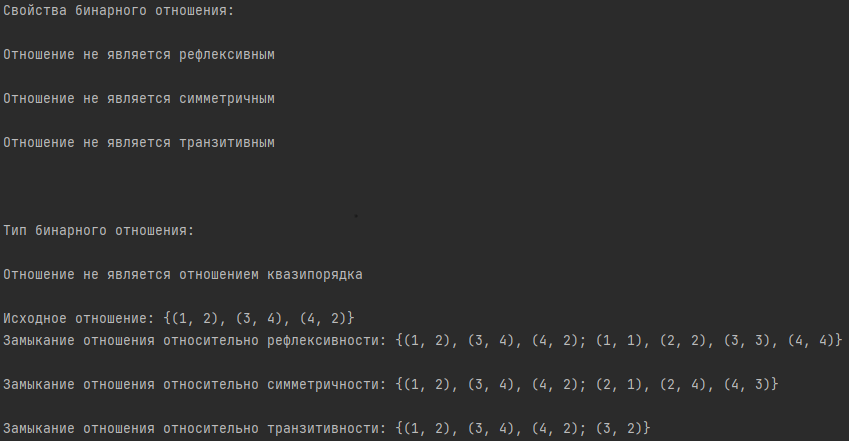
\includegraphics[width=0.8\textwidth]{pic/1.png}
            \caption{}
        \end{figure}
    
    \subsection{Код программы, реализующей рассмотренные алгоритмы}
    
        \inputminted[linenos,breaklines=true, fontsize=\small, style=bw]{python}{code/lab1.py}

    
    \subsection{Оценка сложности реализованных алгоритмов в программе}
    

    \subsubsection{Алгоритм проверки рефлексивности и антирефлексивности}

    Как было сказано в теоретической части лабораторной работы, для проверки 
    отношения на рефлексивность, требуется один проход по главной диагонали
    матрицы отношения, для чего требуется $O(N)$ операций.

    \subsubsection{Алгоритмы проверки рефлексивности и антирефлексивности}

    Как было сказано в теоретической части лабораторной работы, для проверки 
    отношения на свойства рефлексивности и антирефлексивности,требуется один 
    проход по главной диагонали матрицы отношения, для чего требуется $O(N)$ 
    операций.

    \subsubsection{Алгоритмы проверки симметричности и антисимметричности}
    Для проверки отношения на свойства симметричности и антисимметричности 
    в худшем случае требуется полный проход по всем элементам матрицы
    отношения, что составляет $O(N^2)$ операций.

    \subsubsection{Алгоритм проверки транзитивности}
    Для проверки отношения на свойство транзитивности требуется выполнить обход 
    по всем элементам матрицы отношения (для чего требуется один внещний кикл 
    и один вложенный) для всех фиксированных элементов из множества $A$.
    Поэтому асимптотическая оценка данного алгоритма равна $O(N^3)$ операций.

    \subsubsection{Алгоритм классификации}
    Время работы алгоритма классификации в худшем случае составляет 
    $O(N^3 + N^2 + 1)=O(N^3)$.
    

    \subsubsection{Алгоритм построения рефлексивного замыкания}
    Время работы алгоритма составляет $O(N)$

    \subsubsection{Алгоритм построения симметричного замыкания}
    Время работы алгоритма составляет $O(N^2)$

    \subsubsection{Алгоритм построения транзитивного замыкания}
    Время работы алгоритма составляет $O(N^3)$


\conclusion
В ходе лабораторной работы были рассмотрены основные свойства бинарных отношений:
рефлексивность, антирефлексивность, симметричность, антисимметричность и 
транзитивность. По определенным комбинациям свойств отношений, их можно 
классифицировать, как отношения квазипорядка (если отношение обладает 
свойствами транзитивности и рефлексивности), эквивалентности (если отношение 
является отношением квазипорядка, а также имеет свойство симметричности), а 
также отношения частичного порядка (если отношение является отношением 
квазипорядка и имеет свойство антисимметричности). Также были разработаны 
алгоритмы определения свойств отношений и их классификации. В ходе работы стало 
понятно, что самым ресурсоемким стал алгоритм определения транзитивности 
отношения, так как его реализация включает в себя тройной вложенный цикл.

\end{document}